\documentclass[a4paper,10pt]{report}
\usepackage{booktabs}
\renewcommand{\arraystretch}{1.3}
%----------------------------------------------------------------------------------------
%	FONT
%----------------------------------------------------------------------------------------
\usepackage[utf8]{inputenc}
\usepackage[T1]{fontenc}

%\usepackage[scaled=0.8]{beramono} % beramono or luximono give very nice ttfamily fonts

%----------------------------------------------------------------------------------------
%	PAGE LAYOUT
%----------------------------------------------------------------------------------------
\usepackage[toc,page]{appendix}

\textwidth = 410pt

\usepackage{fancyhdr}
\pagestyle{fancy}


\fancyhf{}

%\renewcommand{\sectionmark}[1]{\markright{\thesection.\ #1}}

%\nouppercase{\rightmark}

\lhead{\bfseries \nouppercase{\leftmark}}
\rhead{\bfseries \nouppercase{\rightmark}}
\lfoot{}
\rfoot{\bfseries Page \thepage}

\headwidth=1.1\textwidth
\renewcommand{\headrulewidth}{1.5pt}
\renewcommand{\footrulewidth}{1.5pt}
\fancyhfoffset[L]{24pt}
\fancyhfoffset[R]{24pt}

\fancypagestyle{plain}{%
\fancyhf{} % clear all header and footer fields
\headwidth=1.1\textwidth
\renewcommand{\headrulewidth}{1.5pt}
\renewcommand{\footrulewidth}{1.5pt}
\lhead{\bfseries \nouppercase{\leftmark}}
\rhead{\bfseries \nouppercase{\rightmark}}
%\lhead{\leftmark}
%\rhead{\rightmark}
\lfoot{}
\rfoot{\bfseries Page \thepage}
%\rfoot{Page \thepage}
\headwidth=1.1\textwidth
\fancyhfoffset[L]{24pt}
\fancyhfoffset[R]{24pt}
}

\newcommand{\mysection}[2]{%
                         \sectionmark{#1}%
                         \section{#2}%
                         \sectionmark{#1}%
                       }

%%%%%%%%%
%\renewcommand{\chaptermark}[1]{\markboth{\uppercase{\thechapter.\ #1}}{}}
%\renewcommand{\sectionmark}[1]{\markright{\uppercase{\thesection.\ #1}}}
%\newcommand{\helv}{\fontfamily{phv}\fontseries{b}\fontsize{9}{11}\selectfont}
%\lhead[\helv \thepage]{\helv \rightmark}
%\rhead[\helv \leftmark]{\helv \thepage}
%\cfoot{}
%----------------------------------------------------------------------------------------
%	OTHER PACKAGES and COMMANDS
%----------------------------------------------------------------------------------------
\usepackage{graphicx}
\usepackage{epstopdf}


\usepackage{float}
%\usepackage{tikz}
%\usepackage{tikz-uml} 
\usepackage{amsmath}

\usepackage{pifont}
\usepackage{fourier}
\usepackage{dingbat}

\usepackage{hyperref}

\newcommand{\reffig}[1]{figure \ref{fig:#1}}

\newcommand{\myparagraph}[1]{\paragraph{#1}\mbox{}\\}
%----------------------------------------------------------------------------------------
%	CUSTON LISTING SETTINGS
%----------------------------------------------------------------------------------------
\usepackage{listings}
\usepackage{lstcustom}
\usepackage{enumerate}
\renewcommand{\lstfontfamily}{\ttfamily}
%----------------------------------------------------------------------------------------
%	COLORS
%----------------------------------------------------------------------------------------

\definecolor{Lightgray}{gray}{.80}
\definecolor{lightgrey}{rgb}{0.9,0.9,0.9}


%----------------------------------------------------------------------------------------
%       Commands
%----------------------------------------------------------------------------------------
\newcommand{\Code}[1]{\texttt{#1}}
\newcommand{\BornAgain}{\Code{BornAgain}}%
\newcommand{\IsGISAXS}{\Code{IsGISAXS}}%
\newcommand{\SecLabel}[1]{\label{sec:#1}}%
\newcommand{\SecRef}[1]{Section~\ref{sec:#1}}% 
\newcommand{\MakeRemark}[2]
{ \noindent \smallpencil \colorbox{Lightgray}{\parbox{\dimexpr\linewidth-8\fboxsep}			{\underline{#1} #2 }}
}


%----------------------------------------------------------------------------------------
%	TITLE PAGE
%----------------------------------------------------------------------------------------
\title{
BornAgain - simulating and fitting X-ray and neutron scattering at grazing incidence. \\
\vspace*{10mm} User Guide \\
\large{ version 0.1}
}

\author{Scientific Computing Group at FRM-II}

\usepackage{eso-pic}
\newcommand\BackgroundPic{%
\put(0,0){%
\parbox[b][\paperheight]{\paperwidth}{%
\vfill
\centering
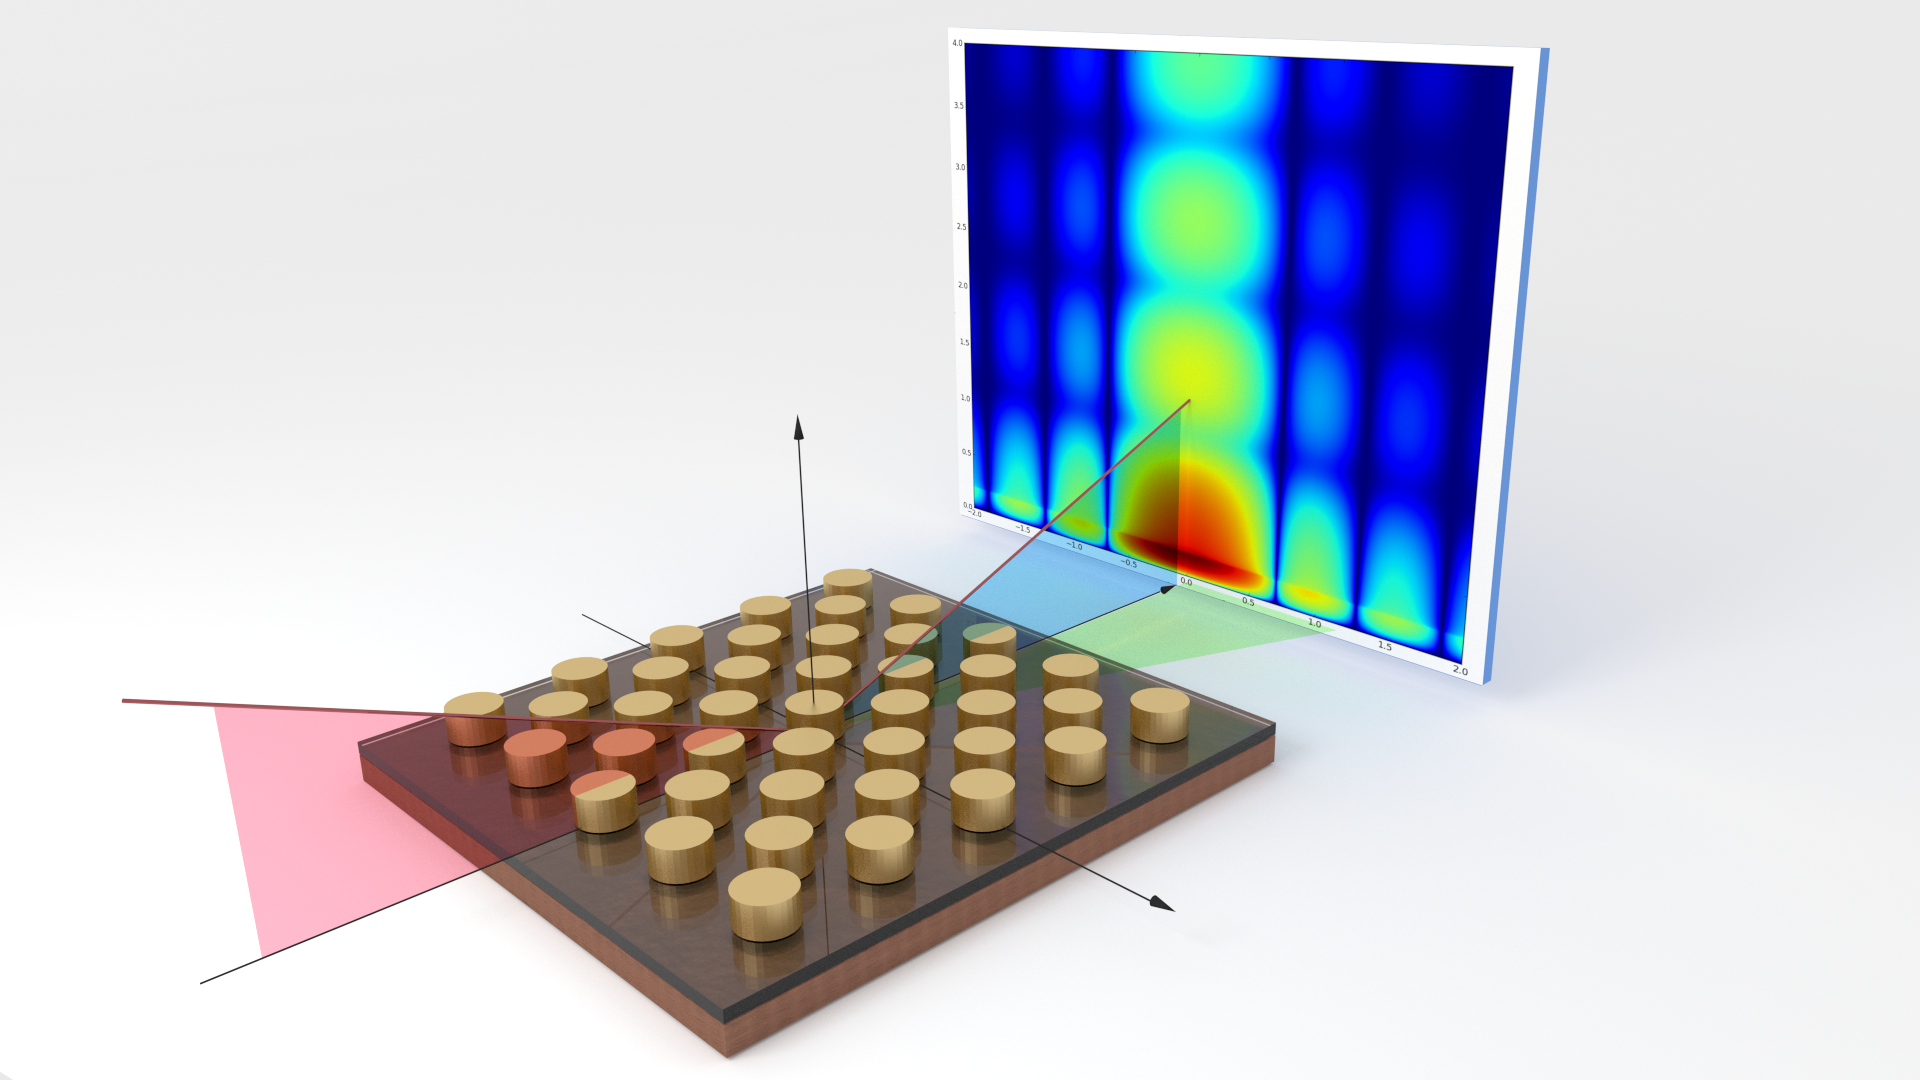
\includegraphics[width=\paperwidth,height=\paperheight,%
keepaspectratio]{results2_2.png}%
\vfill
}}}


%----------------------------------------------------------------------------------------
%	DOCUMENT
%----------------------------------------------------------------------------------------
\begin{document}

\maketitle
\tableofcontents
%\lstlistoflistings
%\listoffigures
%\listoftables

%%%%%%%%%%%%%%%%%%%%%%%%%%%%%%%%%%%%%%%%%%%%%%%%%%%%%%%%%%%%%%%%%%%%%%%%%%%%%%%%
%%
%%   BornAgain User Manual
%%
%%   homepage:   http://www.bornagainproject.org
%%
%%   copyright:  Forschungszentrum Jülich GmbH 2015
%%
%%   license:    Creative Commons CC-BY-SA
%%   
%%   authors:    Scientific Computing Group at MLZ Garching
%%               C. Durniak, M. Ganeva, G. Pospelov, W. Van Herck, J. Wuttke
%%
%%%%%%%%%%%%%%%%%%%%%%%%%%%%%%%%%%%%%%%%%%%%%%%%%%%%%%%%%%%%%%%%%%%%%%%%%%%%%%%%


\cleardoublepage
\mychapter{0}{Introduction}

\BornAgain\
%\marginpar{scope}%
is a free and open-source software package
to simulate and fit small-angle
scattering at grazing incidence (GISAS)
with X-rays (GISAXS) or neutrons (GISANS).
It provides a generic framework
for modeling multilayer samples with smooth or
rough interfaces and with various types of embedded nanoparticles.
%\marginpar{name}%
The name, \BornAgain,
alludes to the central role of the distorted-wave Born
approximation (DWBA) in the physical description of the
scattering process.
\index{Distorted-wave Born approximation}

\BornAgain\
%\marginpar{extends \IsGISAXS}
almost completely reproduces the functionality
of the widely used program \IsGISAXS\
\index{IsGISAXS@\IsGISAXS}
\index{Lazzari, R\'emi}
by R\'emi Lazzari \cite{Laz02,Laz08}.
\BornAgain\ goes beyond \IsGISAXS\ by
supporting an unrestricted number of layers and particles, 
diffuse reflection from rough layer interfaces,
particles with inner structures, neutron polarization and magnetic scattering.
Adhering to a strict object-oriented design,
\BornAgain\ provides a solid base for future extensions
in response to specific user needs.

\BornAgain\
%\marginpar{platforms}%
\index{Platform|see {Operating system}}%
\index{Operating system}%
is operating system independent.
We actively support
Linux,
\index{Linux}%
MacOS
\index{MacOS}%
and  Microsoft Windows.
\index{Windows|see {Microsoft Windows}}%
\index{Microsoft Windows}%
%\marginpar{licence}%
It is a free and open source software under
the GNU General Public License (GPL, version 3 or higher).
This documentation is released under the Creative Commons license CC-BY-SA.
When \BornAgain\ is used in preparing scientific papers,
please cite software and manual as follows:
\index{Citation}%
%\marginpar{citation}%
\begin{quote}
C.~Durniak, M.~Ganeva, G.~Pospelov, W.~Van Herck, J.~Wuttke (2015),\newline
BornAgain --- Software for simulating and fitting
X-ray and neutron small-angle scattering at grazing incidence,
version \UserManualVersionNumber,\newline
\url{http://www.bornagainproject.org}
\end{quote}

This User Manual is complementary to the online documentation
at \url{http://www.bornagainproject.org}.
It does not duplicate information that is more conveniently read online.
Therefore, Sect.~\ref{sec:online} just contains a few pointers to the web site.
The remainder of this User Manual mostly contains background
on the sample models and on the scattering theory implemented in \BornAgain,
and some documentation of the corresponding \Python\ functions.
%Sect.~\ref{sec:Simulation} describes
%the general methodology of a simulation with \BornAgain,
%and gives detailed usage examples.
%Sect.~\ref{sec:ScatteringCrosssection} explains
%which sample structures are supported in \BornAgain,
%and which physical approximations are used.
%Fitting is explained in Sect.~\ref{sec:Fitting}.
%More theoretical background is given in Appendix~\ref{app:theory}.
%Implemented particle formfactors are specified in Appendix~\ref{app:ff}.

\Warn{\indent Software and documentation are work in progress.
We cannot guarantee that they are accurate and correct.
Anyway, it is entirely in the responsibility of users
to ensure that their data interpretation is physically meaningful.
If in doubt, please contact us.}

\index{Bug reports}
We are grateful for all kind of feedback:
criticism, praise, bug reports, feature requests or contributed modules.
If questions go beyond normal user support,
we will be glad to discuss a scientific collaboration.

\newpage
\section{Quick start} \SecLabel{QuickStart}

This section shortly describes how to build \BornAgain\ from source and run first
simulation. More details about software architecture and installation
procedure are given in \SecRef{SoftwareArchitecture} and \SecRef{InstallationProcedure}. \\

\noindent
{\bf Step I: $~$ installing third party software}
\begin{itemize}
\item boost library ($\geq 1.48$)
\item GNU scientific library ($\geq 1.15$)
\item fftw3 library ($\geq 3.3.1$)
\item python-2.7, python-devel, python-numpy-devel
\item Eigen3 library ($\geq 3.1.0$), optional
\item ROOT framework ($\geq 5.34.00$), optional
\item python-matplotlib, optional
\end{itemize}
\vspace*{2mm}


\noindent
{\bf Step II: $~$ getting the source}
\begin{lstlisting}[language=bash, style=commandline]
git clone git://apps.jcns.fz-juelich.de/BornAgain.git 
\end{lstlisting}
\vspace*{3mm}


\noindent
{\bf Step III: $~$ building the source}
\begin{lstlisting}[language=shell, style=commandline]
mkdir <build_dir>; cd <build_dir>;
cmake <source_dir> -DCMAKE_INSTALL_PREFIX=<install_dir>
make
make check
make install
\end{lstlisting}
\vspace*{3mm}


\noindent
{\bf Step IV: $~$ running example}
\begin{lstlisting}[language=shell, style=commandline]
cd <install_dir>/Examples/python/ex001_CylindersAndPrisms
python CylindersAndPrisms.py
\end{lstlisting}


%Requirements

%Hardware
%BornAgain is known to work on following platforms:
%Linux (x86, amd64)
%MacOS X (x86)

%Software
%GCC 4.1.2 or above   C/C++ compiler
%or
%clang
%gcc 4.1.2 or above, clang

\newpage
\chapter{Software architecture}\SecLabel{SoftwareArchitecture}
 

\BornAgain\ is written on C++
and uses object oriented approach to 
achieve modularity, extensibility and transparency.
This leads to the task driven rather then command driven approach in 
different aspects  of the simulation and fitting of GISAS data.
User defines the sample structure, beam and detector characteristics,
fit parameters, using building
blocks -- \Code{classes} -- defined in kernel libraries of the framework.
These buildings blocks are combined together by the user according to his current
task using one the following approach.
\begin{itemize}
\item User imports \BornAgain\ libraries into the python to extent it
with \BornAgain\ API and then prepare python script with sample description and simulation settings. 
User runs the simulation by executing script in python interpreter and then assess
simulation results using the way he likes, e.g. python + numpy + matplotlib.
\item User may construct standalone C++ application linked to \BornAgain\ libraries.
\item User interacts with the framework through graphical 
user drag-and-drop interface (forthcoming).
\end{itemize}

Object oriented approach in the simulation design allows 
to reach much higher level of flexibility in sample construction, 
decouple interdependence in internal calculations and so facilitate creation of new models
that entails little or no modification to the existing code. 


\begin{figure}[htbp]
\centering
  \resizebox{0.9\textwidth}{!}{%
    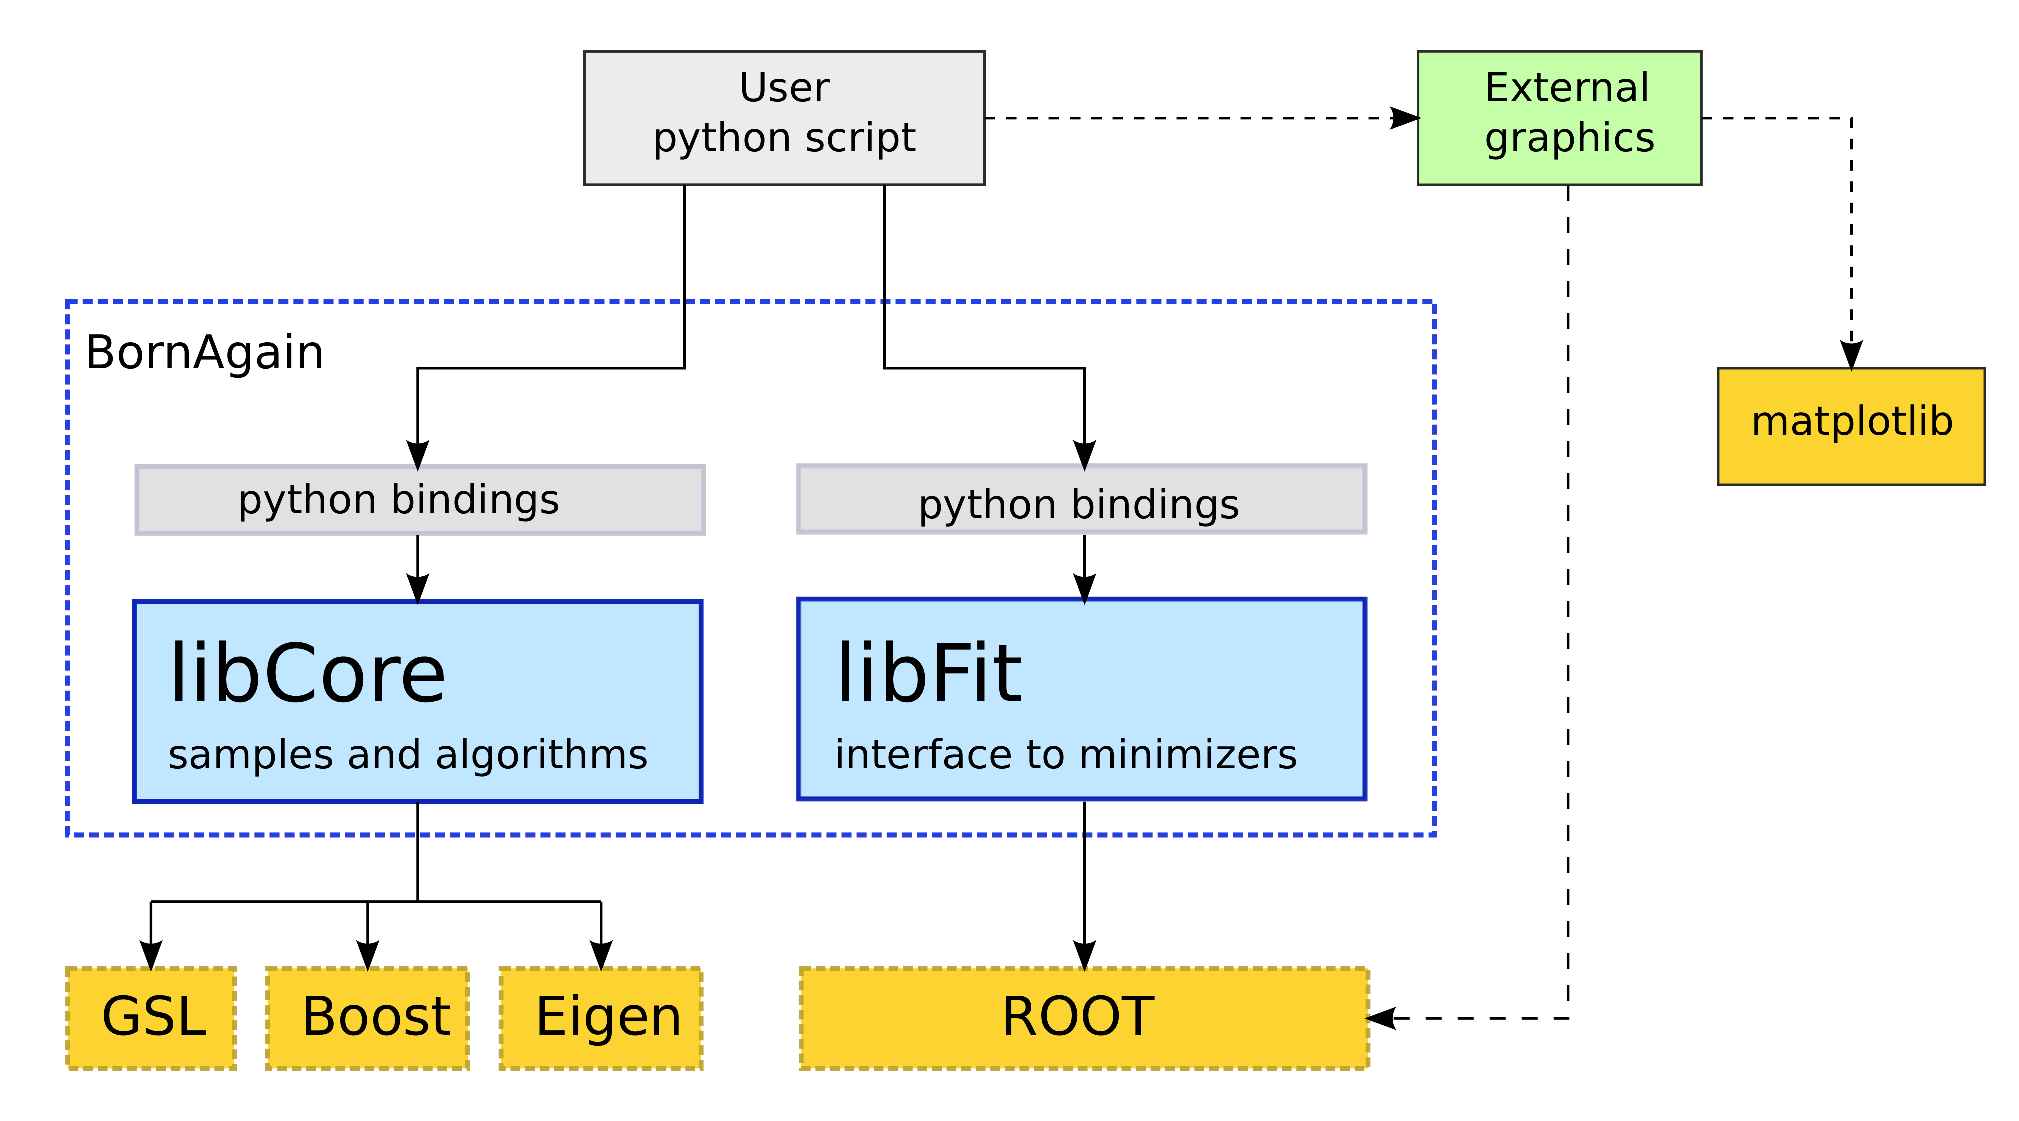
\includegraphics{Figures/basic_architecture.eps}}
\caption{
Structure of \BornAgain\ libraries.
}
\label{fig:two_ratios}
\end{figure}


The general structure of \BornAgain\ and the way user interacts with it are
shown in Fig.~\ref{fig:two_ratios}.
The framework kernel consists of two shared libraries, \Code{libCore} and
\Code{libFit}. Thanks to the python interface they can be imported to the python as external modules. The library \Code{libCore} contains a number of classes, grouped into several class categories necessary for the description of model and running the simulation.
The library  \Code{libFit} contains a number of minimization engines 
and interfaces to them, to let user to fit real data with the model defined.

\BornAgain\ depends from a few external well established open-source libraries: boost, GNU scientific library, Eigen and Fast Fourier Transformation libraries. They are required to be present on the system to run \BornAgain . Other libraries shown
on the plot (ROOT, matplotlib) are optional.

 



\section{Design overview}

% general considerations
% general capabilities and properties
% openess 
% global structure
% design and architecture

% Software process
% - configuration and release management
% - quality assurance and testing
% - user support process


% The BornAgain framework provides a number of classes, grouped into several class categories.


\newpage
\section{Installation} \SecLabel{Installation}

This section describes how to build and install \BornAgain\ libraries from the source.
At the moment we support building on x86/x86\_64 Linux and Mac OS X operating systems.
Support for Windows systems is planned in next releases.
%In the later releases we are planing to include support for Windows systems and provide
%binary distributions for major Windows/Mac/Linux.
There are three major steps to building \BornAgain\ :
\begin{enumerate}[1.]
\item Acquire required third-party libraries.
\item Get \BornAgain\ source code.
\item Use \Code{cmake} to build and install software.
\end{enumerate}
The remainder of this section explains each step in detail.

\subsection{Third-party software.}
To successfully build \BornAgain\ a number of prerequisite packages must be installed.

\begin{itemize}
\item compilers: clang  versions $\geq 3.1$ or GCC versions $\geq 4.2$
\item cmake ($\geq 2.8$)
\item boost library ($\geq 1.48$)
\item GNU scientific library ($\geq 1.15$)
\item fftw3 library ($\geq 3.3$)
\item python ($\geq 2.7$), python-devel, python-numpy-devel
\end{itemize}
\vspace*{2mm}

Other packages are optional
\begin{itemize}
\item ROOT framework (adds several additional fitting algorithms to \BornAgain)
\item python-matplotlib (allows to run usage examples with graphics)
%\item Eigen3 library ($\geq 3.1.0$)
\end{itemize}

All required packages can be easily installed on most Linux distributions using the system's package
manager. Below we give a few examples for several selected operation systems. Please note,
that other distributions (Fedora, Mint, etc) may have different commands for invoking the package manager and slightly different names of packages (like ``boost'' instead of ``libboost'' etc). Besides that, the installation should be very similar.
\vspace*{3mm}

% ---------------
%  OpenSuse 12.3
% ---------------
\noindent
{\large\bf OpenSuse 12.3} \newline
Adding ``scientific'' repository 
\begin{lstlisting}[language=shell, style=commandline]
sudo zypper ar http://download.opensuse.org/repositories/science/openSUSE_12.3 science
\end{lstlisting}

\noindent
Installing required packages
\begin{lstlisting}[language=shell, style=commandline]
sudo zypper install git-core cmake gsl-devel boost-devel fftw3-devel python-devel python-numpy-devel
\end{lstlisting}

\noindent
Installing optional packages
\begin{lstlisting}[language=shell, style=commandline]
sudo zypper install libroot-* root-plugin-* root-system-* root-ttf libeigen3-devel python-matplotlib
\end{lstlisting}
\vspace*{3mm}


% ---------------
%  Ubuntu 13.04
% ---------------
\noindent
{\large\bf Ubuntu 13.04} \newline
Installing required packages
\begin{lstlisting}[language=shell, style=commandline]
sudo apt-get install git cmake libgsl0-dev libboost-all-dev libfftw3-dev python-dev python-numpy
\end{lstlisting}

\noindent
Installing optional packages
\begin{lstlisting}[language=shell, style=commandline]
sudo apt-get install libroot-* root-plugin-* root-system-* ttf-root-installer libeigen3-dev python-matplotlib python-matplotlib-tk
\end{lstlisting}
\vspace*{3mm}


% ---------------
%  MacOS 10.8
% ---------------
\noindent
\noindent
{\large\bf Mac OS X 10.8} \newline
To simplify the installation of third party open-source software on a Mac OS X system we recommend the use of \Code{MacPorts} package manager. 
The easiest way to install MacPorts is by downloading the \Code{dmg} 
from \url{www.macports.org/install.php} and running the system's installer.
After the installation new command ``\Code{port}'' will be available in terminal window of your Mac. \

\noindent
Installing required packages
\begin{lstlisting}[language=shell, style=commandline]
sudo port -v selfupdate
sudo port install git-core cmake
sudo port install fftw-3 gsl
sudo port install boost -no_single-no_static+python27 


\end{lstlisting}

\noindent
Installing optional packages
\begin{lstlisting}[language=shell, style=commandline]
sudo port install py27-matplotlib py27-numpy py27-scipy
sudo port install root +fftw3+python27
sudo port install eigen3
\end{lstlisting}




\subsection{Getting source code}
\BornAgain\ source can be downloaded at \url{http://apps.jcns.fz-juelich.de/BornAgain}
and unpacked with
\begin{lstlisting}[language=shell, style=commandline]
tar xfz bornagain-<version>.tgz
\end{lstlisting}

\noindent
Alternatively one can obtain \BornAgain\ source from our public Git repository.
\begin{lstlisting}[language=bash, style=commandline]
git clone git://apps.jcns.fz-juelich.de/BornAgain.git 
\end{lstlisting}
\vspace*{3mm}


\noindent
{\bf\large More about Git} \\
Our Git repository holds two main branches called ``master'' and ``develop''. We consider ``master''
branch to be the main branch where the source code of HEAD always reflects latest stable release. \Code{git clone} command shown above
\begin{enumerate}[1.]
\item gives you a source code snapshot corresponding to the latest stable release,
\item automatically sets up your local master branch to track our remote master branch, 
so you will be able to fetch changes from the remote branch at any time using ``git pull'' command.
\end{enumerate}

Master branch is updating approximately once per month.
% that reflects our release cycle.
The second branch, ``develop'' branch, is a snapshot of the current development.
This is where any automatic nightly builds are built from. The develop branch is
always expected to work, so to get the most recent features one can switch source code to it by
\begin{lstlisting}[language=bash, style=commandline]
cd BornAgain
git checkout develop
git pull
\end{lstlisting}
\vspace*{3mm}



\subsection{Building and installing the code}

\BornAgain\ should be build using \Code{CMake} cross platform build system. 
Having third-party libraries installed on the system and \BornAgain\ source code acquired as was explained in
previous sections, type build commands
\begin{lstlisting}[language=bash, style=commandline]
mkdir <build_dir>
cd <build_dir>
cmake <source_dir> -DCMAKE_INSTALL_PREFIX=<install_dir>
make
\end{lstlisting}
\vspace*{3mm}

Here \Code{<source\_dir>} is the name of directory, where \BornAgain\ source code has been
copied, \Code{<install\_dir>} is the directory, where user wants  the package
to be installed, and \Code{<build\_dir>} is the directory where building will occur.

\MakeRemark{About \Code{CMake}}{
\\Having dedicated directory \Code{<build\_dir>} for build process
is recommended by \Code{CMake}. That allows several builds with different compilers/options from the same source and keeps source directory clean from build remnants. \\
}


Compilation process invoked by the command ``make'' lasts about 10 min for an average laptop
of 2012 edition. On multi-core machines the compilation time  can be decreased by invoking command
``make'' with the parameter ``make -j[N]'', where N is the number of cores.

Running functional tests is an optional but recommended step. Command ``make check''
will compile several additional tests and run them one by one. Every test contains
the simulation of a typical GISAS geometry and the comparison on numerical level of simulation results with reference files. Having 100\% tests passed ensures that your local installation
is correct.
\begin{lstlisting}[language=bash, style=commandline]
make check
...
100% tests passed, 0 tests failed out of 26
Total Test time (real) = 89.19 sec
[100%] Build target check
\end{lstlisting}
\vspace*{3mm}


The last command ``make install'' copies compiled libraries and some usage examples
into  the installation directory.
\begin{lstlisting}[language=bash, style=commandline]
make install
\end{lstlisting}


\subsubsection{Troubleshooting}

In the case of complex system setup, with variety of libraries of different versions 
scattered across multiple places (\Code{/opt/local}, \Code{/usr} etc.),
you may want to help \Code{CMake} to find libraries in proper place. 
In example below
two system variables are defined to force \Code{CMake} to prefer libraries
found in \Code{/opt/local} to other places.
\begin{lstlisting}[language=bash, style=commandline]
export CMAKE_LIBRARY_PATH=/opt/local/lib:$CMAKE_LIBRARY_PATH
export CMAKE_INCLUDE_PATH=/opt/local/include:$CMAKE_INCLUDE_PATH
\end{lstlisting}


If compilation fails for some reason, please submit your bug report including compilation errors
at \url{http://apps.jcns.fz-juelich.de/redmine/projects/bornagain/issues}



\subsection{What is next?}

In your installation directory you will find
\begin{lstlisting}[language=bash, style=commandline]
./include - header files for compilation of your C++ program
./lib - libraries to import into python or link with your C++ program
./Examples - directory with examples
\end{lstlisting}

Run your first example and enjoy first BornAgain simulation plot.
\begin{lstlisting}[language=bash, style=commandline]
cd <install_dir>/Examples/python/ex001_CylindersAndPrisms
python CylindersAndPrisms.py
\end{lstlisting}








%\newpage
\chapter{Examples} \label{Exampleschap}
%\section{Examples}

\section{General methodology}
A simulation of GISAXS using \BornAgain\ platform can be decomposed into the following points:
\begin{itemize}
\item definition of the materials by specifying their names and their
  refractive indices,
\item definition of particles: shapes, sizes, constituting materials, interference functions,
\item definition of the layers: thicknesses, roughnesses, associations with the previously defined
materials,
\item inclusion of the particles in layers: density, positions, orientations, 
\item assembling the sample: generation of a multilayered system,
\item specifying the input beam and the detector's
  characteristics,
\item running the simulation,
\item saving the data.
\end{itemize}

\noindent The sample is built from object oriented building blocks instead of loading data files.

\section{Conventions}

\subsection{Geometry of the sample}

\noindent The geometry used to describe the sample is shown in \reffig{multil3d}. The $z$-axis is perpendicular to the sample's
surface and pointing upwards. The $x$-axis  is perpendicular to the
plane of the detector and the $y$-axis is along it. The input and the
scattered output beams are each characterized by two angles
$\alpha_i$, $\phi_i$ and $\alpha_f$, $\phi_f$ respectively. Our choice of orientation for the
angles $\alpha_i$ and $\alpha_f$ is so that they are positive as shown in \reffig{multil3d}. \\


\noindent The layers are defined by their thicknesses (parallel to the
$z$-direction), their possible
roughnesses (equal to 0 by default) and the
material they are made of. We do not define any dimensions in the $x$, $y$
directions. And, except for roughness, the layer's vertical boundaries are plane and
perpendicular to the $z$-axis. There is also no limitation to the
number of layers that could be defined in \BornAgain. Note that the
thickness of the top and bottom layer are not defined. \\

\ImportantPoint{Remark:}{- Order of the different steps for the simulation: \\
When assembling the sample, the layers are defined from top to
bottom. So in most cases the first layer will be the air layer.}\\

\noindent The particles are characterized by their form factors (\textit{i.e.} the Fourier transform of the shape function - see the list of form factors implemented
  in \BornAgain) and the composing material. The number of input parameters for the form
  factor depends on the
  particle symmetry; it ranges from one parameter for a sphere (its
  radius) to three for an ellipsoid (its three main axis lengths).\\ By
  placing the particles
inside or on top of a layer, we impose their vertical positions, whose
values corresponds to the bottoms of the particles. The in-plane distribution of particles is linked with the way the
particles interfere with each other, which is therefore implemented
when dealing with the interference function. \\

%\ImportantPoint{Remark:}{Depth of particles\\
%The vertical positions of particles in a layer are given in relative
%coordinates. For the top layer, the bottom corresponds to
%\texttt{depth}=0. But for all the other layers, it is the top of the
%layer which corresponds to \texttt{depth}=0.}\\

\noindent The complex refractive index associated with a layer or a particle is written as $n=1-\delta +i\beta$, with
$\delta, \beta \in \mathbb{R}$. In our program, we input $\delta$ and
$\beta$ directly.

\begin{figure}[h]
  \centering
    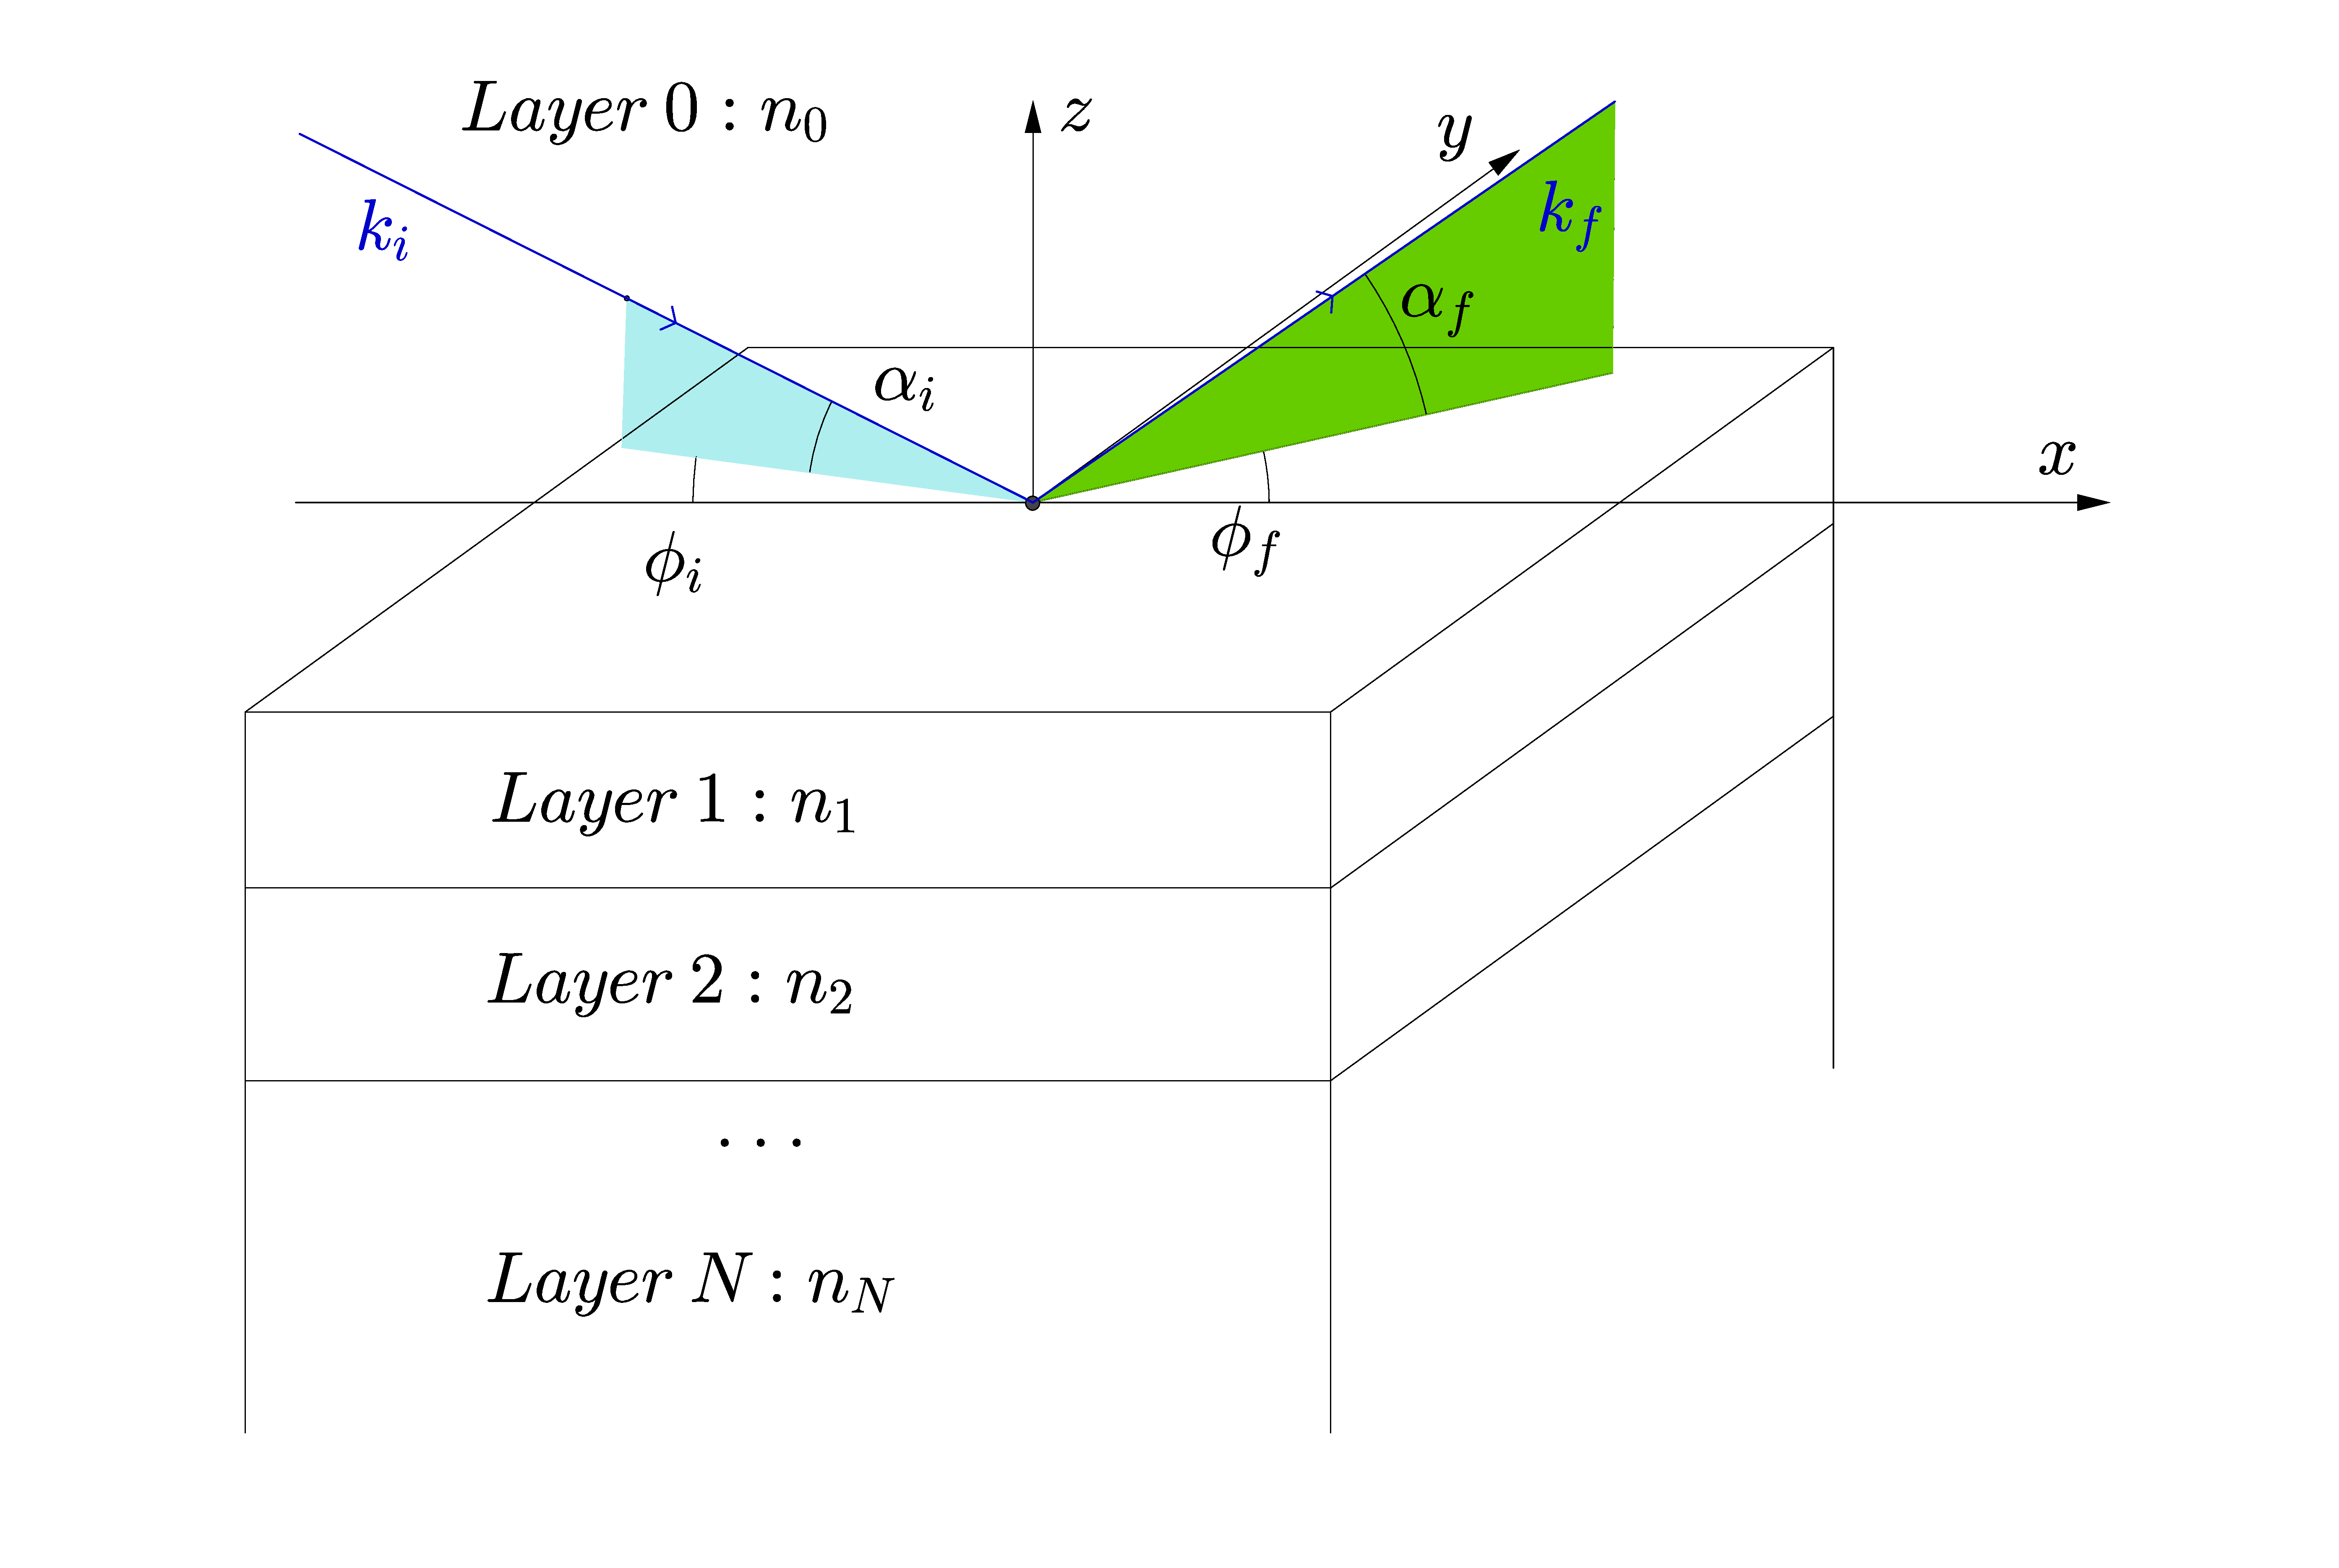
\includegraphics[clip=, width=120mm]{Figures/multilayer3d3.eps}
  \caption[Representation of the scattering geometry.]{Representation of the scattering geometry. $n_j$ is
    the refractive index of layer $j$ and $\alpha_i$ and $\phi_i$ are the incident
    angle of the wave propagating. $\alpha_f$ is the exit angle with respect to the sample's surface and
$\phi_f$ is the scattering angle with respect to the scattering
plane. }
  \label{fig:multil3d}
\end{figure}

\noindent The input beam is assumed to be monochromatic without any
spatial divergence.\\ %\textbf{polarization term?}

\subsection{Units}
By default the angles are expressed in radians and the lengths are given in
nanometers.  But it is possible to use other units by
specifying them right after the value of the corresponding
parameter like, for example, \Code{20.0*micrometer}.


\subsection{Programs}

The examples presented in the next paragraphs are written in Python. For tutorials about this
   programming language, the users are referred to \cite{Pythonref}.

%\noindent Note about the version of C++ and Python to run the examples.\\
%\noindent Where can the following examples be found?\\
%\noindent What is the command to run the examples?

%%%%%%%%%%%%%%%%%%%%%%%%%%%%%%%%%%%%%%%%%%%%
\mysection{Example 1}{Example 1: Two types of islands on top of
  substrate. No interference function} \SecLabel{Example1Python}
% \sectionmark{Example 1}

In this example, we simulate the scattering from a mixture of
cylindrical and prismatic nanoparticles without any interference
between them. These particles are placed in air, on top
of a substrate.\\ We are going to go through each step of the
simulation. The Python script specific to each stage will be given at
the beginning of the description. But for the sake of completeness the full code is given
at the end of this section (Listing~\ref{script_ex1}). \\

\noindent We start by importing different functions from external
modules (line~\ref{import_lib}), for example NumPy, which
is a fundamental package for scientific computing with Python \cite{NumPyURL}.  In particular, line~\ref{import_end}
imports the features of \BornAgain\ software.\\

\begin{lstlisting}[language=python, style=eclipseboxed,name=ex1,nolol]
import sys, os, numpy @\label{import_lib}@

from libBornAgainCore import * @\label{import_end}@
\end{lstlisting}


 %%%%%%%%%%%%%  
\myparagraph{\underline{First step:} Defining materials} 
 

\begin{lstlisting}[language=python, style=eclipseboxed,name=ex1,nolol]
def RunSimulation(): @\label{def_function}@
    #  defining materials @\label{material1}@
    mAmbience = MaterialManager.getHomogeneousMaterial("Air", 0.0, 0.0)  @\label{material2}@
    mSubstrate = MaterialManager.getHomogeneousMaterial("Substrate",
    6e-6, 2e-8) @\label{material3}@
    mParticle = MaterialManager.getHomogeneousMaterial("Particle", 6e-4,
  2e-8 ) @\label{materialparticle}@
\end{lstlisting}

\noindent Line~\ref{def_function} marks the beginning of the
function to define and run the simulation. 

\noindent Lines~\ref{material2}, \ref{material3} and \ref{materialparticle} define different
materials using function \Code{getHomogeneousMaterial} from class
\Code{MaterialManager}. The general syntax is the following 

\begin{lstlisting}[language=python, style=eclipse,numbers=none]
<material_name> = MaterialManager.getHomogeneousMaterial("name", delta, beta)
\end{lstlisting}

\noindent where \Code{name} is the name of the
material associated with its complex refractive index
n=1-\Code{delta} +i \Code{beta}. \Code{<material\_name>} is later used when
referring to this particular material. The three defined materials in this example are \Code{Air} with a refractive
index of 1 (\Code{delta = beta =0}), a \Code{Substrate} associated with a complex refractive index
equal to $1-6\times 10^{-6} +i2\times 10^{-8} $, and the material of particles, whose refractive index is \Code{n}$=1-6\times 10^{-4}+i2\times 10^{-8}$.\\\\

%\noindent \underline{Remark:} there is no condition on the choice of \Code{name}. 
 %%%%%%%%%%%%% 
\myparagraph{\underline{Second step:} Defining the particles} 

\begin{lstlisting}[language=python,style=eclipseboxed,name=ex1,nolol]
    # collection of particles @\label{particles1}@
    cylinder_ff = FormFactorCylinder(5*nanometer, 5*nanometer) @\label{particlescyl1}@
    cylinder = Particle(mParticle, cylinder_ff) @\label{particlescyl2}@
    prism_ff = FormFactorPrism3(5*nanometer, 5*nanometer) @\label{particlesprism1}@
    prism = Particle(mParticle, prism_ff) @\label{particlesprism2}@
\end{lstlisting}

 \noindent We implement two different shapes of particles: cylinders and
 prisms (\textit{i.e.} elongated particles with a constant equilateral triangular cross section).\\ All particles implemented in \BornAgain\ are defined by their
 form factors, their sizes and the material
  they are made of. Here, for the
  cylindrical particle, we input its radius and height.  For the prism, 
  the possible inputs are the length of one side of its equilateral triangular
  base and its height.\\

%\noindent In line~\ref{complx_ref_index}, we define the complex refractive index
%associated with both particle shapes: \Code{n}$=1-6\times 10^{-4}+i2\times 10^{-8}$.\\
  
\noindent In order to define a particle, we proceed in two steps. For example for
the cylindrical particle, we first specify the form factor of a cylinder with 
its radius and height, both equal to 5 nanometers in this particular
case (see line~\ref{particlescyl1}). Then we associate this shape with
the constituting material as in line~\ref{particlescyl2}.\\

\noindent The same procedure has been applied for the prism in lines~\ref{particlesprism1} and \ref{particlesprism2} respectively.
 %%%%%%%%%%%%% 
\myparagraph{\underline{Third step:} Characterizing the layers and assembling the sample} 

\noindent \textbf{Particle decoration} \\
  

\begin{lstlisting}[language=python, style=eclipseboxed, name=ex1,nolol]
    particle_decoration = ParticleDecoration()  @\label{particlesdecor1}@
    particle_decoration.addParticle(cylinder, 0.0, 0.5)  @\label{particlesdecor2}@
    particle_decoration.addParticle(prism, 0.0, 0.5)@\label{particlesdecor3}@
    interference = InterferenceFunctionNone()  @\label{particlesnointerf}@
    particle_decoration.addInterferenceFunction(interference)  @\label{particlesinterf}@
\end{lstlisting}

\noindent The object which holds the information about the positions and densities of particles
in our sample is called \Code{ParticleDecoration}
(line~\ref{particlesdecor1}). We use the associated function \Code{addParticle}
for each particle shape (lines~\ref{particlesdecor2}, \ref{particlesdecor3}). Its general
syntax is 

\begin{lstlisting}[language=python, style=eclipse,numbers=none]
addParticle(<particle_name>, depth, abundance) 
\end{lstlisting}

\noindent  where \Code{<particle\_name>} is the name used to define the particles
(lines~\ref{particlescyl2} and \ref{particlesprism2}), \Code{depth}
(default value =0)
is the vertical position, expressed in nanometers, of the particles in a given layer (the
association with a particular layer will be done during the next step) and
\Code{abundance} is the proportion of this type of particles, 
normalized to the total number of particles. Here we have 50\% of cylinders
and 50\% of prisms. \\ 

\ImportantPoint{Remark:}{Depth of particles\\
The vertical positions of particles in a layer are given in relative
coordinates. For the top layer, the bottom corresponds to
\Code{depth}=0 and negative values would correspond to particles
floating above layer 1 since the vertical axis, shown in \reffig{multil3d} is pointing upwards. But for all the other layers, it is the top of the
layer which corresponds to \Code{depth}=0.}\\


\noindent Finally lines~\ref{particlesnointerf} and
\ref{particlesinterf} specify that there is \textbf{no coherent interference} between
the waves scattered by these particles. The intensity is calculated by
the incoherent sum of the scattered waves: $\langle |F_n|^2\rangle$,
where $F_n$ is the form factor associated with the particle of type $n$.  The way these waves
interfere imposes the horizontal distribution of
the particles as
the interference reflects the long or short-range order of the
particles distribution (\textbf{see Theory}). On the contrary, the vertical position is
imposed when we add the particles in a given layer by parameter \Code{depth}, as shown in lines~\ref{particlesdecor2} and \ref{particlesdecor3}. \\

\noindent \textbf{Multilayer}\\
  
\begin{lstlisting}[language=python, style=eclipseboxed,name=ex1,nolol]
    # air layer with particles and substrate form multi layer  @\label{sampleassembling}@
    air_layer = Layer(mAmbience)  @\label{airlayer}@
    air_layer.setDecoration(particle_decoration)  @\label{airlayerdecorator}@
    substrate_layer = Layer(mSubstrate, 0)  @\label{substratelayer}@
    multi_layer = MultiLayer()  @\label{multilayercanvas}@
    multi_layer.addLayer(air_layer)  @\label{layerairdecor}@
    multi_layer.addLayer(substrate_layer)  @\label{layersubstrate}@
\end{lstlisting}

\noindent We now have to configure our sample. For this first example,
the particles, \textit{i.e.} cylinders and prisms, are on top of a substrate in an
air layer. \textbf{The order in which we define these layers is important: we
start from the top layer down to the bottom one}.\\

\noindent Let us start with the air layer. It contains the particles. In
line~\ref{airlayer}, we use the previously defined \Code{mAmbience}
(="air" material) (line~\ref{material2}). The command written in line~\ref{airlayerdecorator} shows that this layer is decorated by adding the
particles using the function \Code{particle\_decoration} defined in
lines~\ref{particlesdecor1}-\ref{particlesinterf}. The substrate layer
only contains the substrate material (line~\ref{substratelayer}).\\%Note that the
%\Code{depth} is referenced to the bottom of the top layer (negative
%values would correspond to particles floating above layer 1 as
%the vertical axis is pointing upwards). 
 
\noindent There are different possible syntaxes to define a layer. As shown in
lines~\ref{airlayer} and \ref{substratelayer}, we can use
\Code{Layer(<material\_name>,thickness)} or
\Code{Layer(<material\_name>)}. The second case corresponds
to the default value of the \Code{thickness}, equal to 0. The \Code{thickness} is
expressed in  nanometers. \\

\noindent Our two layers are now fully characterized. The sample is assembled using
\Code{MultiLayer()} constructor (line~\ref{multilayercanvas}): we start with the air layer decorated
with the particles (line~\ref{layerairdecor}), which is the layer at
the top and end with the bottom layer, which is the
substrate (line~\ref{layersubstrate}).
 %%%%%%%%%%%%% 
\myparagraph{\underline{Fourth step:} Characterizing the input beam and
output detector and running the simulation} 


\begin{lstlisting}[language=python, style=eclipseboxed,name=ex1,nolol]
    # run simulation  @\label{run1}@
    simulation = Simulation()  @\label{run2}@
    simulation.setDetectorParameters(100,-1.0*degree, 1.0*degree, 
                                100, 0.0*degree, 2.0*degree, True)  @\label{rundetector}@
    simulation.setBeamParameters(1.0*angstrom, 0.2*degree, 0.0*degree)  @\label{runbeam}@
    simulation.setSample(multi_layer)  @\label{runsample}@
    simulation.runSimulation()  @\label{runsimul}@
\end{lstlisting}


\noindent The first stage is to define the \Code{Simulation()} object (line~\ref{run2}). Then we define the detector (line~\ref{rundetector}) and beam
parameters (line~\ref{runbeam}), which are associated with the
sample previously defined (line~\ref{runsample}). Finally we run
the simulation (line~\ref{runsimul}). Those functions are part of the Simulation
class.  The
different incident and exit angles are
shown in \reffig{multil3d}. \\

\noindent The detector parameters are set using ranges of angles via
the function:\\

\noindent \Code{setDetectorParameters(n\_phi, phi\_f\_min,
  phi\_f\_max,\\ \phantom{setDetectorParameters(}n\_alpha, alpha\_f\_min, alpha\_f\_max, isgisaxs\_style=false)}, \\

\noindent where \Code{n\_phi=100} is the number of iterations for $\phi_f$,\\ \Code{phi\_f\_min=-1.0*degree} and \Code{phi\_f\_max=1.0*degree}
are the minimum and maximum values respectively of $\phi_f$, \\ \Code{n\_alpha=100} is
the number of iterations for $\alpha_f$,\\ \Code{alpha\_f\_min=0.0*degree} and \Code{alpha\_f\_max=2.0*degree} 
are the minimum and maximum values respectively of
$\alpha_f$. \\
\Code{isgisaxs\_style=True} (default value = \Code{False}) is a boolean
used to characterise the structure of the output data. If
\Code{isgisaxs\_style=True}, the output data is binned at constant
values of the sine of the output angles, $\alpha_f$ and $\phi_f$, otherwise it is binned
at constant values of these two angles.\\


\noindent For the beam the function to use is
\Code{setBeamParameters(lambda, alpha\_i, phi\_i)}, where\\
\Code{lambda=1.0*angstrom} is the incident beam wavelength,
\Code{alpha\_i=0.2*degree} is the incident
grazing angle on the surface of the sample,
\Code{phi\_i=0.0*degree} is the in-plane
direction of the incident beam (measured with respect to the
$x$-axis).\\ 

\noindent \underline{Remark}: Note that, except for
\Code{isgisaxs\_style}, there are no default values implemented for the
parameters of the beam and detector.\\

\noindent Line~\ref{runsimul} shows the command to run the simulation using the
previously defined setup.
%%%%%%%%%%%%%
\myparagraph{\underline{Fifth step:} Saving the data} 


\begin{lstlisting}[language=python, style=eclipseboxed,name=ex1,nolol]
    # retrieving intensity data
    return GetOutputData(simulation) @\label{outputdata}@
\end{lstlisting}


\noindent In line~\ref{outputdata} we obtain the simulated intensity
as a function of outgoing angles $\alpha_f$ and $\phi_f$ for further
uses (plots, fits,\ldots) as a NumPy array containing
\Code{n\_phi}$\times$\Code{n\_alpha}
datapoints. Some options are provided by \BornAgain. For example, \reffig{output_ex1} shows the two-dimensional
contourplot of the intensity as a function of $\alpha_f$ and
$\phi_f$. 

\begin{figure}[h]
  \begin{center}
   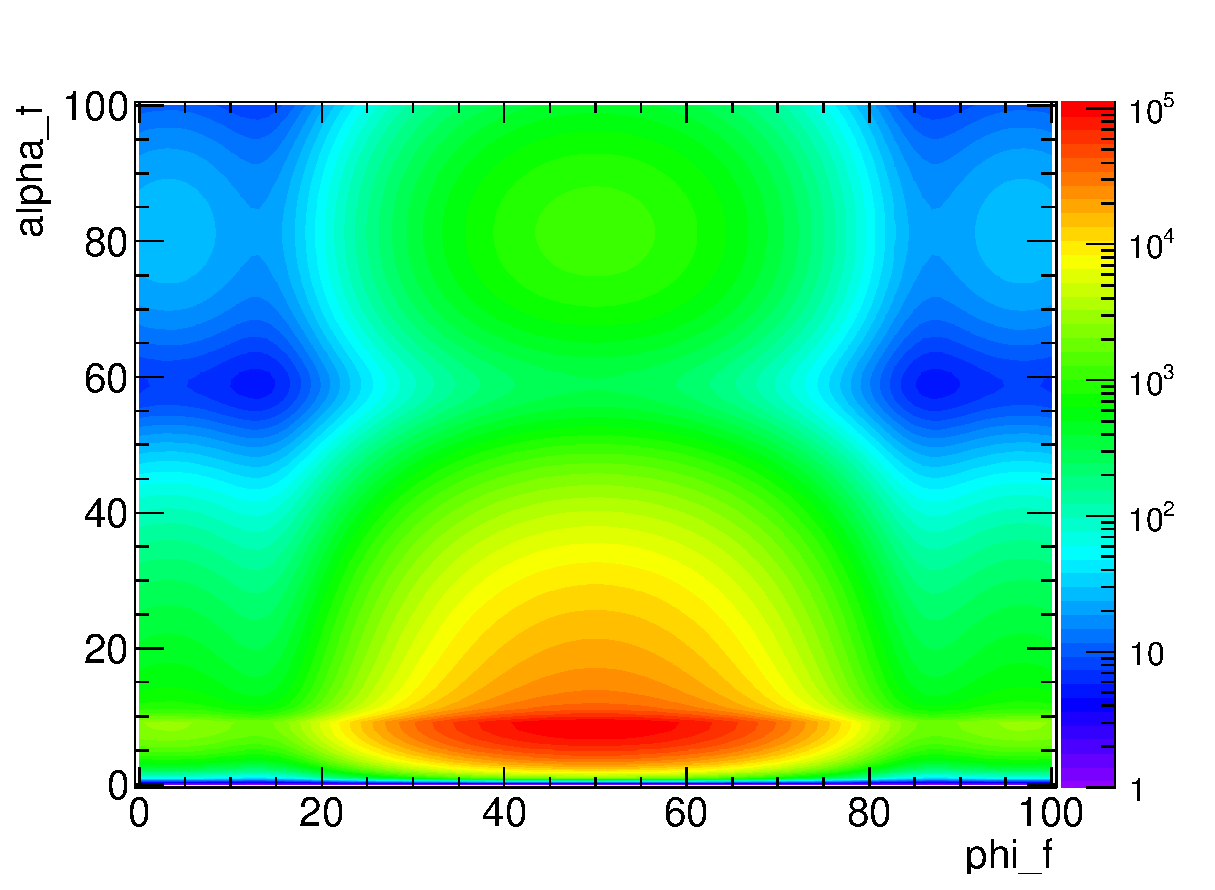
\includegraphics[clip=true, width=120mm]{Figures/Manual_ex1.eps}
  \end{center}
  \caption[Example 1: Simulated grazing-incidence small-angle X-ray scattering from a mixture of
cylindrical and prismatic nanoparticles without any interference, deposited on top
of a substrate]{Figure of example 1: Simulated grazing-incidence small-angle X-ray scattering from a mixture of
cylindrical and prismatic nanoparticles without any interference, deposited on top
of a substrate. The input beam is characterized by a wavelength
$\lambda$ of 1~\AA\ and incident angles $\alpha_i=0.2^{\circ}$, $\phi_i=0^{\circ}$. The
cylinders have a radius and a height both equal to 5~nm, the prisms
are characterized by a side length equal to 5~nm and they are also 5~nm high. The
material of the particles has a refractive index of $1-6\times 10^{-4}+i2\times 10^{-8}$. For the substrate
it is equal to $1-6\times 10^{-6} +i2\times 10^{-8} $. The colorscale
is associated with the output intensity in arbitrary units. }
\label{fig:output_ex1}
\end{figure}

\newpage
\begin{lstlisting}[caption={Python script of example 1},
  label=script_ex1,captionpos=b,escapeinside={@}{@} ,language=python,style=eclipse, numbers= none,frame = leftline ,
      framerule = 2mm ,
      rulecolor = \color{lightgrey},
      breaklines = true]
import sys, os, numpy 

sys.path.append(os.path.abspath(os.path.join(os.path.split(__file__)[0],'..', '..', '..', 'lib')))

from libBornAgainCore import * 

def RunSimulation():
    #  defining materials 
    mAmbience = MaterialManager.getHomogeneousMaterial("Air", 0.0, 0.0 ) 
    mSubstrate = MaterialManager.getHomogeneousMaterial("Substrate",
    6e-6, 2e-8) 
    mParticle = MaterialManager.getHomogeneousMaterial("Particle", 6e-4, 2e-8 )
    # collection of particles 
    cylinder_ff = FormFactorCylinder(5*nanometer, 5*nanometer) 
    cylinder = Particle(mParticle, cylinder_ff) 
    prism_ff = FormFactorPrism3(5*nanometer, 5*nanometer) 
    prism = Particle(mParticle, prism_ff) 
    particle_decoration = ParticleDecoration()  
    particle_decoration.addParticle(cylinder, 0.0, 0.5)  
    particle_decoration.addParticle(prism, 0.0, 0.5)  
    interference = InterferenceFunctionNone()  
    particle_decoration.addInterferenceFunction(interference)  
    # air layer with particles and substrate form multi layer 
    air_layer = Layer(mAmbience)  
    air_layer.setDecoration(particle_decoration)
    substrate_layer = Layer(mSubstrate, 0) 
    multi_layer = MultiLayer()  
    multi_layer.addLayer(air_layer) 
    multi_layer.addLayer(substrate_layer) 

    # build and run simulation  
    simulation = Simulation()  
    simulation.setDetectorParameters(100,-1.0*degree, 1.0*degree, 
                                    100, 0.0*degree, 2.0*degree, True) 
    simulation.setBeamParameters(1.0*angstrom, 0.2*degree, 0.0*degree) 
    simulation.setSample(multi_layer) 
    simulation.runSimulation()  

    # retrieving intensity data
     return GetOutputData(simulation)
\end{lstlisting}

% \newpage
% \subsection{Hello, minted}
% 
% \begin{minted}[linenos=true, frame=single]{python}
% mAmbience = MaterialManager.getHomogeneousMaterial("Air", 1.0, 0.0 )
% mSubstrate = MaterialManager.getHomogeneousMaterial("Substrate", 1.0-6e-6, 2e-8 )
% n_particle = complex(1.0-6e-4, 2e-8)
% cylinder_ff = FormFactorCylinder(5*nanometer, 5*nanometer)
% cylinder = Particle(n_particle, cylinder_ff)
% prism_ff = FormFactorPrism3(5*nanometer, 5*nanometer)
% prism = Particle(n_particle, prism_ff)
% particle_decoration = ParticleDecoration()
% particle_decoration.addParticle(cylinder, 0.0, 0.5)
% particle_decoration.addParticle(prism, 0.0, 0.5)
% interference = InterferenceFunctionNone()
% particle_decoration.addInterferenceFunction(interference)
% # air layer with particles and substrate form multi layer
% air_layer = Layer(mAmbience)
% air_layer_decorator = LayerDecorator(air_layer, particle_decoration)
% substrate_layer = Layer(mSubstrate, 0)
% multi_layer = MultiLayer()
% multi_layer.addLayer(air_layer_decorator)
% multi_layer.addLayer(substrate_layer)
% 
% # build and run experiment
% simulation = Simulation()
% simulation.setDetectorParameters(100,-1.0*degree, 1.0*degree, 100, 0.0*degree, 2.0*degree, True)
% simulation.setBeamParameters(1.0*angstrom, -0.2*degree, 0.0*degree)
% simulation.setSample(multi_layer)
% simulation.runSimulation()
% \end{minted}

\section{Example 2}





%List of notations\\  Bugs\\ License agreement\\ Directory layout \\ FAQ \\ Future development.

%\appendix
%%Appendix
\chapter{Implemented classes}

\begin{itemize}
\item Particle decoration
\item Layer
\item MultiLayer
\item Simulation
\end{itemize}

\chapter{Form factors}
% plots of particles + orientation of the axes
% plots of the form factors

\begin{itemize}
\item Parallelepiped (\texttt{FormFactorParallelepiped})

\begin{equation}
F() = 4H R^2\exp(i q_z H/2) \frac{sin(q_xR)}{q_x R}\frac{ \sin(q_yR)}{q_y R}\frac{\sin(q_z H/2)}{q_z H/2}
\end{equation}
\item Pyramid (\texttt{FormFactorPyramid})

\begin{align*}
        q_1 &=(H/2)((q_x-q_y)/\tan(\alpha) + q_z)\\
        q_2 &=(H/2)((q_x-q_y)/\tan(\alpha) - q_z)\\
        q_3 &=(H/2)((q_x+q_y)/\tan(\alpha) + q_z) \\
        q_4 &=(H/2)((q_x+q_y)/\tan(\alpha) - q_z)\\
        K_1 &= \frac{\sin(q_1)}{q_1} \exp(i q_1)  + i \frac{\sin(q_2)}{q_2} \exp(-i q_2)\\
        K_2 &= -i \frac{sin(q_1)}{q_1} exp(i q_1) +i \frac{\sin(q_2)}{q_2} \exp(-i q_2)\\
        K_3 &= \frac{\sin(q_3)}{q_3}\exp(i q_3)    + \frac{\sin(q_4)}{q_4} \exp(-i q_4)\\
        K_4 &= -i \frac{\sin(q_3)}{q_3} \exp(i q_3) + i \frac{\sin(q_4)}{q_4} \exp(-i q_4)\\     
  F() &= \frac{H}{q_x q_y} [ K_1 \cos( (q_x-q_y)R ) + K_2 \sin( (q_x-q_y)R ) - K_3 \cos( (q_x+q_y) R ) - K_4 \sin( (q_x+q_y) R )]
   \end{align*}
	
\item Cylinder (\texttt{FormFactorCylinder})

  \begin{equation}
 F()=   H  \frac{\sin(q_ z H/2)}{q_z H/2} \exp(i q_ z H/2) 2\pi R^2 \frac{J_1(|q_{\parallel} R |)}{|q_{\parallel} R| }
 \end{equation}
 

\item Prism3 (\texttt{FormFactorPrism3})

\begin{equation}
    F()= 2 \sqrt{3}\frac{\exp(-i q_y R/\sqrt{3})}{q_x^2-3q_y^2}[\exp(i \sqrt{3} q_y R ) -\cos(q_x R)-i \sqrt{3} q_y R \frac{\sin(q_x R)}{q_x R}]   H \frac{\sin(q_z H/2 )}{q_z H/2} \exp(i q_z H/2)
\end{equation}

\item Sphere (\texttt{FormFactorSphere})

\begin{equation}    
return 2\pi \exp(i q_z (H-R))\int_{R-H} ^{R} R_z^2 \frac{J_1(|q_p*R_z|) }{|q_p*R_z|}
        \exp(i q_z*Z)
\end{equation}


\item Full sphere (\texttt{FormFactorFullSphere})

\begin{equation}
radial = 4\pi R^3*\frac{\sin(q R) - q R*\cos(q R)}{(qR)^3}
\end{equation}

\item Box (\texttt{FormFactorBox})

\begin{equation}
F()= 4H R W\exp(i q_z H/2) \frac{\sin(q_x R)}{q_x R} \frac{  \sin(q_y W) }{q_y W}\frac{\sin(q_z H/2)}{q_z H/2}
\end{equation}
    
	
\end{itemize}

\chapter{Interference functions}

\begin{itemize}
\item	No interference 
\item	decoupling approximation 	
\item 	local mono disperse approximation 
\item 	size spacing approximation 
\end{itemize}


\chapter{Pair correlation functions}
\begin{itemize}
\item The Debye hard core 
\item The gaussian
\item The Lennard-Jonnes  	
\item The gate pair correlation 	
\item The Debye hard core with power-law decrease  	
\item The Zhu pair correlation function 	
\item The Venables pair correlation function 	
\item The bidimensional hard core pair function.
\end{itemize}	

\bibliography{ref}
\bibliographystyle{unsrt}


\end{document}

